\documentclass[11pt]{article}
% ===========================================================================
%  Shared preamble for all MPM2D worksheets — input right after \documentclass.
%  (Files beginning with "_" are skipped by mpm2d-worksheet-publish.mjs.)
% ===========================================================================
\usepackage[letterpaper,top=2.2cm,bottom=1.9cm,left=1.6cm,right=1.6cm,headheight=28pt,footskip=24pt]{geometry}
\usepackage{amsmath,amssymb}
\usepackage[T1]{fontenc}
\usepackage[utf8]{inputenc}
\usepackage{lmodern}
\usepackage{xcolor}
\usepackage[most]{tcolorbox}
\usepackage{enumitem}
\usepackage{multicol}
\usepackage{fancyhdr}
\usepackage{tikz}
\usetikzlibrary{calc}
\usepackage{pgfplots}
\pgfplotsset{compat=1.18}

\definecolor{exblue}{HTML}{4A90E2}
\definecolor{exbg}{HTML}{E6F3FF}
\definecolor{qorange}{HTML}{E69138}
\definecolor{qbg}{HTML}{FFF7CC}
\definecolor{keygray}{HTML}{475569}
\definecolor{keybg}{HTML}{F1F5F9}
\definecolor{iagreen}{HTML}{14653B}
\definecolor{titleblue}{HTML}{1D4ED8}
% Rotating palette so each worked example gets its own colour.
\definecolor{ex0}{HTML}{2563A0}\definecolor{ex1}{HTML}{3B7D3B}\definecolor{ex2}{HTML}{8A5A00}
\definecolor{ex3}{HTML}{A3327A}\definecolor{ex4}{HTML}{6D28A3}\definecolor{ex5}{HTML}{B08900}
\definecolor{ex6}{HTML}{0E7490}\definecolor{ex7}{HTML}{9A3412}\definecolor{ex8}{HTML}{15803D}

\pagestyle{fancy}
\fancyhf{}
\fancyhead[L]{\footnotesize NAME: \underline{\hspace{3.4cm}}}
\fancyhead[C]{\textbf{Integration Academy}\\[-2pt]{\scriptsize Math Simplified \textperiodcentered{} Success Amplified}}
\fancyhead[R]{\footnotesize MPM2D}
\fancyfoot[L]{\scriptsize dr.merie@IntegrationAcademy.ca}
\fancyfoot[C]{\scriptsize\thepage}
\fancyfoot[R]{\scriptsize IntegrationAcademy.ca}
\renewcommand{\headrulewidth}{1.2pt}
\renewcommand{\footrulewidth}{0.4pt}
\setlength{\parindent}{0pt}
\setlength{\parskip}{4pt}

% Examples are NOT breakable, so each example + its solution stays on one page.
\newtcolorbox{example}[2]{colframe=#1,colback=#1!7,coltitle=white,colbacktitle=#1,fonttitle=\bfseries,title={#2},arc=3pt,boxrule=1pt}
\newtcolorbox{qbox}[1]{colframe=qorange,colback=qbg,coltitle=white,colbacktitle=qorange,fonttitle=\bfseries,title={#1},arc=3pt,breakable,boxrule=1pt}
\newtcolorbox{keybox}{colframe=keygray,colback=keybg,coltitle=white,colbacktitle=keygray,fonttitle=\bfseries,title={$\checkmark$\ Answer Key},arc=3pt,breakable,boxrule=1pt}
\newtcolorbox{recapbox}{colframe=keygray,colback=keybg,coltitle=white,colbacktitle=keygray,fonttitle=\bfseries,title={Question Recap},arc=3pt,breakable,boxrule=1pt}
\newtcolorbox{ideabox}{colframe=titleblue,colback=titleblue!6,coltitle=white,colbacktitle=titleblue,fonttitle=\bfseries,title={The Big Ideas},arc=3pt,breakable,boxrule=1.2pt}
\newtcolorbox{learnbox}{colframe=iagreen,colback=iagreen!5,coltitle=white,colbacktitle=iagreen,fonttitle=\bfseries,title={Core Concepts},arc=3pt,breakable,boxrule=1.2pt}
\newcommand{\lh}[1]{\par\smallskip{\bfseries\color{iagreen}#1}\par\nobreak\smallskip}

\newcommand{\soln}{\par\smallskip\textit{\textbf{Solution.}}\ }
\newcommand{\workspace}[1]{\par\vspace{3pt}\fcolorbox{black!30}{white}{\begin{minipage}[t][#1][t]{\dimexpr\linewidth-2\fboxsep\relax}\ \end{minipage}}\par}
\newcommand{\sech}[1]{\par\vspace{8pt}{\Large\bfseries\color{iagreen}#1}\par\nobreak\vspace{2pt}{\color{black!20}\hrule height1pt}\vspace{6pt}}

% A compact coordinate plot sized for an example box: \eplot{xmin}{xmax}{ymin}{ymax}{body}
\newcommand{\eplot}[5]{\begin{center}\begin{tikzpicture}
\begin{axis}[width=6.8cm,height=4.4cm,axis lines=middle,xlabel={\tiny$x$},ylabel={\tiny$y$},
grid=both,grid style={gray!16},xmin=#1,xmax=#2,ymin=#3,ymax=#4,
xtick distance=2,ytick distance=2,tick label style={font=\tiny},axis line style={-},samples=120]
#5
\end{axis}\end{tikzpicture}\end{center}}

% Same as \eplot but with its own tick spacing: \eplotx{xmin}{xmax}{ymin}{ymax}{xtick}{ytick}{body}
\newcommand{\eplotx}[7]{\begin{center}\begin{tikzpicture}
\begin{axis}[width=8.4cm,height=5.4cm,axis lines=middle,xlabel={\tiny$x$},ylabel={\tiny$y$},
grid=both,grid style={gray!16},xmin=#1,xmax=#2,ymin=#3,ymax=#4,
xtick distance=#5,ytick distance=#6,tick label style={font=\tiny},axis line style={-},samples=120]
#7
\end{axis}\end{tikzpicture}\end{center}}

% A sine-curve plot (degrees on x, 0..360): \splot{ymin}{ymax}{body}
\newcommand{\splot}[3]{\begin{center}\begin{tikzpicture}
\begin{axis}[width=8.6cm,height=4.6cm,axis lines=middle,xlabel={\tiny$x\,(^\circ)$},ylabel={\tiny$y$},
grid=both,grid style={gray!16},xmin=0,xmax=360,ymin=#1,ymax=#2,
xtick distance=90,ytick distance=1,tick label style={font=\tiny},axis line style={-},samples=180]
#3
\end{axis}\end{tikzpicture}\end{center}}

% A small coordinate plot: \plot{xmin}{xmax}{ymin}{ymax}{body}
\newcommand{\plot}[5]{\begin{center}\begin{tikzpicture}
\begin{axis}[width=8.4cm,height=6cm,axis lines=middle,xlabel={\scriptsize$x$},ylabel={\scriptsize$y$},
grid=both,grid style={gray!16},xmin=#1,xmax=#2,ymin=#3,ymax=#4,
xtick distance=2,ytick distance=2,tick label style={font=\tiny},axis line style={-}]
#5
\end{axis}\end{tikzpicture}\end{center}}

% Right triangle (angle theta at bottom-left, right angle at bottom-right):
%   \rtri{drawBase}{drawHeight}{oppLabel}{adjLabel}{hypLabel}
\newcommand{\rtri}[5]{\begin{center}\begin{tikzpicture}[scale=0.85]
\coordinate (A) at (0,0);\coordinate (B) at (#1,0);\coordinate (C) at (#1,#2);
\draw[thick,exblue] (A)--(B)--(C)--cycle;
\draw[black] ($(B)+(-0.32,0)$)--($(B)+(-0.32,0.32)$)--($(B)+(0,0.32)$);
\node[below] at ($(A)!0.5!(B)$){#4};
\node[right] at ($(B)!0.5!(C)$){#3};
\node[above left] at ($(A)!0.5!(C)$){#5};
\node at (0.7,0.22){$\theta$};
\end{tikzpicture}\end{center}}

% General (oblique) triangle with vertex labels and opposite-side labels:
%   \gtri{Alabel}{Blabel}{Clabel}{aSide}{bSide}{cSide}
\newcommand{\gtri}[6]{\begin{center}\begin{tikzpicture}[scale=0.85]
\coordinate (A) at (0,0);\coordinate (B) at (5,0);\coordinate (C) at (1.6,3);
\draw[thick,exblue] (A)--(B)--(C)--cycle;
\node[below left] at (A){#1};\node[below right] at (B){#2};\node[above] at (C){#3};
\node[below] at ($(A)!0.5!(B)$){#6};
\node[right] at ($(B)!0.5!(C)$){#4};
\node[left] at ($(A)!0.5!(C)$){#5};
\end{tikzpicture}\end{center}}

\fancyhead[R]{\footnotesize MHF4U \textperiodcentered{} 3.3}
\begin{document}

\begin{center}
{\LARGE\bfseries\color{titleblue}Worksheet 3.3 --- Solving Rational Equations \& Inequalities}\\[2pt]
{\small Grade 12 Advanced Functions (MHF4U) \textperiodcentered{} Unit 3: Rational Functions}
\end{center}

\begin{ideabox}
Clear fractions with the LCD and check restrictions; for inequalities, find the critical values (zeros of numerator and denominator) and use a sign chart.
\begin{itemize}[leftmargin=*,itemsep=2pt]
  \item Equation: multiply by the LCD, solve, reject extraneous roots.
  \item Inequality: get $0$ on one side, find critical values, test intervals.
  \item Denominator zeros are always excluded (open circles).
\end{itemize}
\end{ideabox}

\begin{learnbox}
\lh{Clear the denominators}Solve a rational equation by multiplying through by the common denominator, then solving the resulting polynomial equation.
\lh{Check restrictions}Any value that makes an original denominator zero is not allowed, so reject such extraneous solutions.
\lh{Inequalities need a sign chart}For a rational inequality, use the zeros of the numerator \emph{and} the denominator to build a sign chart across the intervals.
\end{learnbox}

\sech{Worked Examples}

\begin{example}{ex0}{Example 1 --- Simple equation}
Solve $\dfrac1x=2$.\soln $1=2x\Rightarrow x=\tfrac12$.
\end{example}

\begin{example}{ex1}{Example 2 --- Cross-multiply}
Solve $\dfrac{x+3}{x-1}=4$.\soln $x+3=4(x-1)=4x-4\Rightarrow 7=3x\Rightarrow x=\tfrac73$ (valid).
\end{example}

\begin{example}{ex2}{Example 3 --- Clear the LCD}
Solve $\dfrac9x+1=4$.\soln $\dfrac9x=3\Rightarrow 9=3x\Rightarrow x=3$.
\end{example}

\begin{example}{ex3}{Example 4 --- Inequality}
Solve $\dfrac{x+1}{x-3}>0$.\soln Critical values $-1,3$; signs $+,-,+$. So $x<-1$ or $x>3$:\begin{center}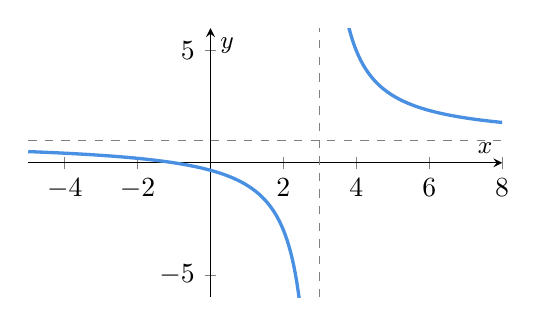
\begin{tikzpicture}\begin{axis}[width=7.6cm,height=5cm,axis lines=middle,xlabel={\small$x$},ylabel={\small$y$},xmin=-5,xmax=8,ymin=-6,ymax=6,samples=160,restrict y to domain=-7:7]\addplot[exblue,very thick,domain=-5:2.82]{(x+1)/(x-3)};\addplot[exblue,very thick,domain=3.18:8]{(x+1)/(x-3)};\draw[dashed,gray] (axis cs:3,-6)--(axis cs:3,6);\draw[dashed,gray] (axis cs:-5,1)--(axis cs:8,1);\end{axis}\end{tikzpicture}\end{center}
\end{example}

\begin{example}{ex4}{Example 5 --- Reciprocal inequality}
Solve $\dfrac{1}{x-5}<0$.\soln Negative when $x-5<0$, so $x<5$.
\end{example}

\begin{example}{ex5}{Example 6 --- Cross-multiply}
Solve $\dfrac{2x-1}{x+2}=3$.\soln $2x-1=3(x+2)=3x+6\Rightarrow x=-7$ (valid).
\end{example}

\begin{example}{ex6}{Example 7 --- Clear the LCD}
Solve $\dfrac{12}x-1=2$.\soln $\dfrac{12}x=3\Rightarrow x=4$.
\end{example}

\begin{example}{ex7}{Example 8 --- Inequality}
Solve $\dfrac{x-4}{x}>0$.\soln Critical values $0,4$; signs $+,-,+$: $x<0$ or $x>4$.
\end{example}

\begin{example}{ex8}{Example 9 --- Reciprocal inequality}
Solve $\dfrac{1}{3-x}>0$.\soln Positive when $3-x>0$, so $x<3$.
\end{example}

\clearpage
\sech{Your Turn --- Show Your Work}
For each question, show all steps clearly in the space provided.

\begin{qbox}{Question 1}
Solve $\dfrac7x=2$.\workspace{2.4cm}
\end{qbox}

\begin{qbox}{Question 2}
Solve $\dfrac{x+4}{x-1}=5$.\workspace{2.4cm}
\end{qbox}

\begin{qbox}{Question 3}
Solve $\dfrac{10}x-3=2$.\workspace{2.4cm}
\end{qbox}

\begin{qbox}{Question 4}
Solve $\dfrac{x}{x+6}>0$.\workspace{2.4cm}
\end{qbox}

\begin{qbox}{Question 5}
Solve $\dfrac{-1}{x+2}>0$.\workspace{2.4cm}
\end{qbox}

\begin{qbox}{Question 6}
Solve $\dfrac5x=10$.\workspace{2.4cm}
\end{qbox}

\begin{qbox}{Question 7}
Solve $\dfrac{x+2}{x-1}=3$.\workspace{2.4cm}
\end{qbox}

\begin{qbox}{Question 8}
Solve $\dfrac6x+2=5$.\workspace{2.4cm}
\end{qbox}

\begin{qbox}{Question 9}
Solve $\dfrac{x}{x-3}<0$.\workspace{2.4cm}
\end{qbox}

\begin{qbox}{Question 10}
Solve $\dfrac{1}{x-4}>0$.\workspace{2.4cm}
\end{qbox}

\begin{qbox}{Question 11}
Solve $\dfrac{2}{x}=\dfrac{1}{x-1}$.\workspace{2.4cm}
\end{qbox}

\begin{qbox}{Question 12}
Solve $\dfrac{x-2}{x+1}\ge0$.\workspace{2.4cm}
\end{qbox}

\begin{qbox}{Question 13 --- Challenge}
Solve $\dfrac{x+1}{x-2}\le0$ using critical values.\workspace{3.5cm}
\end{qbox}

\clearpage
\sech{Question Recap \& Answer Key}

\begin{recapbox}
\begin{multicols}{2}
\small
\begin{enumerate}[leftmargin=*,itemsep=3pt]
  \item Solve $\dfrac7x=2$.
  \item Solve $\dfrac{x+4}{x-1}=5$.
  \item Solve $\dfrac{10}x-3=2$.
  \item Solve $\dfrac{x}{x+6}>0$.
  \item Solve $\dfrac{-1}{x+2}>0$.
  \item Solve $\dfrac5x=10$.
  \item Solve $\dfrac{x+2}{x-1}=3$.
  \item Solve $\dfrac6x+2=5$.
  \item Solve $\dfrac{x}{x-3}<0$.
  \item Solve $\dfrac{1}{x-4}>0$.
  \item Solve $\dfrac{2}{x}=\dfrac{1}{x-1}$.
  \item Solve $\dfrac{x-2}{x+1}\ge0$.
  \item Solve $\dfrac{x+1}{x-2}\le0$ using critical values.
\end{enumerate}
\end{multicols}
\end{recapbox}

\begin{keybox}
\begin{multicols}{2}
\small
\begin{enumerate}[leftmargin=*,itemsep=3pt]
  \item $x=\tfrac72$
  \item $x=\tfrac94$
  \item $x=2$
  \item $x<-6$ or $x>0$
  \item $x<-2$
  \item $x=\tfrac12$
  \item $x=\tfrac52$
  \item $x=2$
  \item $0<x<3$
  \item $x>4$
  \item $x=2$
  \item $x\le-1$ or $x>2$
  \item $-1\le x<2$
\end{enumerate}
\end{multicols}
\end{keybox}

\end{document}
